\documentclass[../lecture-notes.tex]{subfiles}

\begin{document}

    \subsection{Circom Walkthrough}

    In this final lecture, we bridge the gap between the theoretical concepts presented in previous lectures and their practical realization using the \textbf{Circom} DSL.

    \begin{definition}
        \textbf{Circom} is a domain-specific language for building arithmetic circuits that can be used to produce zk-SNARK proofs.
    \end{definition}

    Throughout this lecture, we will walk through how concepts like R1CS, witness, trusted setup, and verification keys appear in actual code and practice.

    \subsubsection{Journey Begins}

    In the previous lectures, we covered a variety of theoretical concepts: zk-SNARKs, trusted setup, arithmetic circuits, constraints, witnesses, and the Rank-1 Constraint System (R1CS) representation.
    Now, let's see how these appear in practice.

    \subsubsection{From Theory to Practice: Circom}

    We learned that a circuit can represent a complex arithmetic computation over a finite field.
    Circom allows us to write these circuits in a high-level syntax.
    To begin, consider the arithmetic circuit $r = x \times y$.

    It can be represented in Circom syntax as follows:

    \begin{lstlisting}[language=Circom]
    pragma circom 2.1.6;

    template Math() {
        signal input x;
        signal input y;

        signal output r <== x * y;
    }

    component main = Math();
    \end{lstlisting}

    Here, we see how easy it is to define a circuit that takes two inputs $x,y$ and outputs their product $r$.
    The \texttt{template} defines a reusable circuit component, while \texttt{signal input} and \texttt{signal output} represent inputs and outputs, respectively.
    Intermediate signals (without \texttt{input} or \texttt{output}) are internal primitives within the circuit.

    \textbf{Public vs Private Signals:}

    Output signals are always public.
    You may also define public inputs by specifying them in the main component, for example:

    \begin{lstlisting}[language=Circom,numbers=none]
    component main {public [x]} = Math();
    \end{lstlisting}

    This means $x$ is a public input and will appear in the verification context.
    The order of public signals in the final proof verification step follows the order of their definition inside the template, starting with outputs.

    \newpage

    For example, if your circuit looks like this:
    \begin{lstlisting}[language=Circom]
    template Circuit() {
        signal x;

        signal output o2;

        signal input c;
        signal input a;

        signal k1;

        signal input b;

        signal output o1;
    }

    component main {public [a, b, c]} = Circuit();
    \end{lstlisting}

    The order of the public signals that should be passed to the verifier is as follows:
    \[ (\texttt{o2}, \texttt{o1}, \texttt{c}, \texttt{a}, \texttt{b}) \]

    \subsubsection{Arguments, Functions, and Vars}

    Sometimes we need to calculate some values as constants for our circuit.
    For example, if you want your circuit to be a multi-tool that, based on provided arguments, can work with different cases.
    For this purpose, we can declare \textit{functions} and \textit{vars} inside the circuit, as shown below:

    \begin{lstlisting}[language=Circom]
    function transformNumber(value) {
        return value ** 2;
    }

    template Math(padding) {
        signal input x;
        signal input y;

        var elementsNumber = transformNumber(padding);
        signal b <== x * elementsNumber;

        signal output r <== b * y;
    }

    component main {public [x]} = Math(12);
    \end{lstlisting}

    Here, \texttt{var elementsNumber} and the function \\ \texttt{transformNumber}
    are evaluated at compile time. Remember that assignments using \texttt{var} and
    functions do not produce constraints by themselves. Only \texttt{<==},
    \texttt{==>}, or \texttt{===} and actual arithmetic on signals produce
    constraints reflected in R1CS.

    \begin{remark}
        Sometimes, one needs to perform operations like division or non-quadratic multiplication on the signal.
        For this purpose, you can use the \texttt{{-}->} and \texttt{<-{-}} notations to compute the values ``out-of-circuit''. For example:

        \begin{lstlisting}[language=Circom,numbers=none]
template Math() {
    signal input x;
    signal input y;

    signal b <-- x / y;

    signal output r <== b * y;
}

component main = Math();
        \end{lstlisting}\label{code:division-example}

        In this case, no constraints are generated with the $x$ input, and it does not even participate in the witness directly.

        \textcolor{green!50!black}{\textbf{Notice!}} This is the main difference between Circom and other languages. When you
        write a function evaluation $y = f(x)$ in any other language (say, Python or Rust),
        you are specifying the set of instructions to compute $y$ from $x$ (commonly
        sequentially). In Circom (or in any other R1CS language) you are merely asserting
        the \textbf{correctness} of the computation and therefore of all
        intermediate computations. This way, if your task would have been to compute
        $y = \frac{1}{x}$, you could simply ask $y$ to be the result of the division
        (that can be computed out of circuit) and then asserting that $x \times y = 1$
        with $x \neq 0$. This way, you are not writing the division itself, but
        the constraints that the division should satisfy.
    \end{remark}

    \subsubsection{Theoretical Recap: Using the Learned Concepts}

    Next, let us apply the learned concepts to a more complex examples. We start
    with the \texttt{if} statement logic.

    \begin{example}
        Recall the complex example we analyzed in earlier lectures:

        \begin{lstlisting}[language=Python,numbers=none]
def r(x1: bool, x2: F, x3: F) -> F:
    return x2 * x3 if x1 else x2 + x3
        \end{lstlisting}

        This can be represented as:
        \[
            r = x_1 \times (x_2 \times x_3) + (1 - x_1) \times (x_2 + x_3).
        \]

        We also had the additional constraint $x_1 \times (1 - x_1) = 0$ to ensure $x_1$ is binary.

        The resulting system of constraints was:
        \begin{gather*}
            x_1 \times x_1 = x_1 \tag{1}\\
            x_2 \times x_3 = \mathsf{mult} \tag{2}\\
            x_1 \times \mathsf{mult} = \mathsf{selectMult} \tag{3}\\
            (1 - x_1) \times (x_2 + x_3) = r - \mathsf{selectMult} \tag{4}\\
        \end{gather*}
    \end{example}

    It took us quite some time to understand and come up with the constraint system, which can be visualized as follows:

    \begin{figure}[h!]
        \centering
        \scalebox{0.5}{
        \begin{tikzpicture}
            \colorlet{circle edge}{gray!50!black}
            \colorlet{circle area}{gray!20}
            \colorlet{gate1 edge}{green!50!black}
            \colorlet{gate1 area}{green!20}
            \colorlet{gate2 edge}{orange!50!black}
            \colorlet{gate2 area}{orange!20}
            \colorlet{gate3 edge}{blue!50!black}
            \colorlet{gate3 area}{blue!20}

            \tikzset{
                var/.style={circle, draw=circle edge, fill=circle area, very thick, minimum size=1cm, text centered},
                gate1/.style={circle, draw=gate1 edge, fill=gate1 area, ultra thick, minimum size=1cm, text centered},
                gate2/.style={circle, draw=gate2 edge, fill=gate2 area, ultra thick, minimum size=1cm, text centered},
                gate3/.style={circle, draw=gate3 edge, fill=gate3 area, ultra thick, minimum size=1cm, text centered},
                arrow/.style={-Stealth, ultra thick}
            }

            % Nodes
            \node[var] (c) at (0, -3) {$c$};
            \node[var] (b) at (0, -1.5) {$b$};
            \node[var] (a) at (0, 0) {$a$};
            \node[var] (one) at (0, 1.5) {$1$};

            % b+c and b*c gates
            \node[gate1] (b_plus_c) at (3, -1.5) {$+$};
            \node[gate2] (b_times_c) at (3, -3.0) {$\times$};

            \node[gate3] (one_minus_a) at (3, 0.75) {$-$};

            % a*b*c and (1-a)(b+c) gates
            \node[gate2] (a_times_b_times_c) at (6, -2.0) {$\times$};
            \node[gate2] (one_minus_a_times_b_plus_c) at (6, -0.5) {$\times$};

            % a*b*c + (1-a)(b+c) gate
            \node[gate1] (r) at (9, -1.25) {$+$};

            % Result node
            \node[var] (result) at (11.5, -1.25) {$r$};

            % b+c and b*c arrows
            \draw[arrow,gray] (b) to (b_plus_c);
            \draw[arrow,gray] (b) to (b_times_c);
            \draw[arrow,gray] (c) to (b_plus_c);
            \draw[arrow,gray] (c) to (b_times_c);

            % 1 - c arrow
            \draw[arrow,gray] (one) to (one_minus_a);
            \draw[arrow,gray] (a) to (one_minus_a);

            % a*b*c and (1-a)(b+c) arrows
            \draw[arrow,gray] (a) to [bend left=20] (a_times_b_times_c);
            \draw[arrow,gray] (b_times_c) to node[midway, above] {$r_1$} (a_times_b_times_c);
            \draw[arrow,gray] (one_minus_a) to node[midway, above] {$r_3$} (one_minus_a_times_b_plus_c);
            \draw[arrow,gray] (b_plus_c) to node[midway, above] {$r_2$} (one_minus_a_times_b_plus_c);

            % a*b*c + (1-a)(b+c) arrows
            \draw[arrow,gray] (a_times_b_times_c) to [bend right=20] node[midway, above] {$r_4$} (r);
            \draw[arrow,gray] (one_minus_a_times_b_plus_c) to [bend left=20] node[midway, above] {$r_5$} (r);

            % Result arrow
            \draw[arrow,gray!50!black] (r) to (result);

        \end{tikzpicture}
        }
        \caption{Example of a circuit evaluating the \texttt{if} statement logic.}
        \label{fig:polynomial-circuit}
    \end{figure}

    The inputs can be directly transformed into signals like below:
    \begin{lstlisting}[language=Circom]
    template Math() {
        signal output r;

        signal input x1;

        signal input x2;
        signal input x3;
    }
    \end{lstlisting}

    In our case, we have an additional output signal, so we can \texttt{"}return\texttt{"} it from the circuit.
    Now, let's compare the mathematical and Circom representations.

    % FIXME (@ZamDimon): Spacing below is freaking awful. Please fix it later.
    \begin{center}
        \vspace{-2mm}
        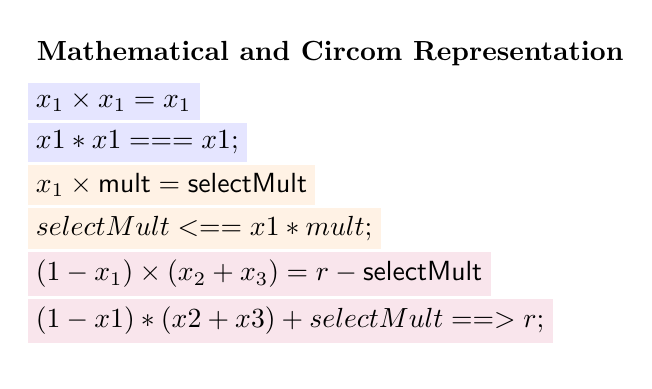
\begin{tikzpicture}
            \node[inner sep=0pt, outer sep=-5mm, align=left] (mathside) at (-4.5,0) {
                \\
                \vspace{1mm}

                \textbf{Mathematical and Circom Representation} \\
                \colorbox{blue!10!white}{$x_1 \times x_1 = x_1$} \\
                \colorbox{blue!10!white}{$x1 * x1 === x1;$} \\
                
                \colorbox{orange!10!white}{$x_1 \times \mathsf{mult} = \mathsf{selectMult}$} \\
                \colorbox{orange!10!white}{$selectMult <== x1 * mult;$} \\
                
                \colorbox{purple!10!white}{$(1 - x_1) \times (x_2 + x_3) = r - \mathsf{selectMult}$} \\
                \colorbox{purple!10!white}{$(1 - x1) * (x2 + x3) + selectMult ==> r;$} \\
            };
        \end{tikzpicture}
        \vspace{-2mm}

    \end{center}

    As we can see, the translation from math to Circom is straightforward.
    We have used \textit{signals} for constraint definitions.

    \begin{remark}
        If you wish to follow along with the explanations in the following chapters:
        \begin{enumerate}
            \item Clone the repository \url{https://github.com/ZKDL-Camp/hardhat-zkit-template}.
            \item Run \texttt{npm install} to install dependencies and \texttt{npx hardhat zkit make}
            to compile Circom circuits and generate the necessary artifacts.
        \end{enumerate}
    \end{remark}

    \subsubsection{From R1CS to Proof Generation}

    Now, let us break down everything that is happening during the proof
    generation process. After compilation, you will find the following files in
    the \texttt{zkit/artifacts/circuits} folder (starting from the project
    root):
    \begin{itemize}
        \item \texttt{.r1cs} file: The Rank-1 Constraint System representation of the circuit.
        \item \texttt{.wasm and *.js} files: The code to compute the witness from the given inputs.
        \item \texttt{.zkey} file: Proving keys after the trusted setup.
        \item \texttt{.sym} file: Symbolic reference for signals.
    \end{itemize}

    \textbf{R1CS File.} Let us start with the \texttt{.r1cs} file. In \Cref{section:circuits},
    we defined the following coefficient vectors (in simple constraints) for our
    task:
    \begin{equation*}
        \scalebox{0.75}{$   
        \begin{aligned}
            \mathbf{a}_1 &= (0, 0, 1, 0, 0, 0, 0) & \quad \mathbf{b}_1 &= (0, 0, 1, 0, 0, 0, 0) & \quad \mathbf{c}_1 &= (0, 0, 1, 0, 0, 0, 0) \\
            \mathbf{a}_2 &= (0, 0, 0, 1, 0, 0, 0) & \quad \mathbf{b}_2 &= (0, 0, 0, 0, 1, 0, 0) & \quad \mathbf{c}_2 &= (0, 0, 0, 0, 0, 1, 0) \\
            \mathbf{a}_3 &= (0, 0, 1, 0, 0, 0, 0) & \quad \mathbf{b}_3 &= (0, 0, 0, 0, 0, 1, 0) & \quad \mathbf{c}_3 &= (0, 0, 0, 0, 0, 0, 1) \\
            \mathbf{a}_4 &= (1, 0, -1, 0, 0, 0, 0) & \quad \mathbf{b}_4 &= (0, 0, 0, 1, 1, 0, 0) & \quad \mathbf{c}_4 &= (0, 1, 0, 0, 0, 0, -1)
        \end{aligned}
        $}
    \end{equation*}

    On the other hand, using the test from the \\ \texttt{test/Math.witness.test.ts} file and reading the R1CS file, we can see:

    \begin{center}
        \begin{tcolorbox}[enhanced,
            width=1.0\textwidth,
            title={\textbf{test/Math.witness.test.ts}},
            coltitle=gray!25!black,
            attach boxed title to top center={yshift=-2mm,yshifttext=-1mm},
            boxed title style={size=small,colframe=gray!75!black,
            colback=Green!30!white,boxrule=1.5pt},
            top=-0.3cm,
            bottom=-0.3cm]
            \begin{lstlisting}[language=TypeScript,numbers=none,basicstyle=\scriptsize\ttfamily\scriptsize]
    expect(constraint1[0]).to.deep.equal([ 0n, 0n, 1n, 0n, 0n, 0n, 0n ]);
    expect(constraint1[1]).to.deep.equal([ 0n, 0n, 1n, 0n, 0n, 0n, 0n ]);
    expect(constraint1[2]).to.deep.equal([ 0n, 0n, 1n, 0n, 0n, 0n, 0n ]);

    expect(constraint2[0]).to.deep.equal([ 0n, 0n, 0n, babyJub.F.negone, 0n, 0n, 0n ]);
    expect(constraint2[1]).to.deep.equal([ 0n, 0n, 0n, 0n, 1n, 0n, 0n ]);
    expect(constraint2[2]).to.deep.equal([ 0n, 0n, 0n, 0n, 0n, babyJub.F.negone, 0n ]);

    expect(constraint3[0]).to.deep.equal([ 0n, 0n, babyJub.F.negone, 0n, 0n, 0n, 0n ]);
    expect(constraint3[1]).to.deep.equal([ 0n, 0n, 0n, 0n, 0n, 1n, 0n ]);
    expect(constraint3[2]).to.deep.equal([ 0n, 0n, 0n, 0n, 0n, 0n, babyJub.F.negone ]);

    expect(constraint4[0]).to.deep.equal([ babyJub.F.negone, 0n, 0n, 0n, 0n, 0n, 0n ]);
    expect(constraint4[1]).to.deep.equal([ 0n, 0n, 0n, 1n, 0n, 0n, 0n ]);
    expect(constraint4[2]).to.deep.equal([ 0n, babyJub.F.negone, 0n, 0n, 0n, 0n, 0n ]);
            \end{lstlisting}
        \end{tcolorbox}
    \end{center}

    Mostly, the structure generated by Circom aligns with what we had devised, except for the last constraint.
    The difference occurs because of Circom's optimization to make proof generation and verification more efficient.

    Now, let's take a closer look at how the witness is computed. In \Cref{section:circuits}, we had:
    \[ \mathbf{w} = (1, r, x_1, x_2, x_3, \mathsf{mult}, \mathsf{selectMult}) \]

    Given the inputs: $x_1 = 1, x_2 = 3, x_3 = 4$, we can quickly do the math
    and find out that the actual witness should look like this: $\mathbf{w} =
    (1, 12, 1, 3, 4, 12, 12)$ based on:
    \begin{gather*}
        \mathsf{mult} = 3 \times 4 = 12 \\
        \mathsf{selectMult} = 1 \times 12 = 12 \\
        r = 1 \times (3 \times 4) + (1 - 1) \times (3 + 4) = 12 + 0 = 12
    \end{gather*}

    Indeed, it aligns with the test from:

    \begin{center}
        \begin{tcolorbox}[enhanced,
            width=0.75\textwidth,
            title={\textbf{test/Math.witness.test.ts}},
            coltitle=gray!25!black,
            attach boxed title to top center={yshift=-2mm,yshifttext=-1mm},
            boxed title style={size=small,colframe=gray!75!black,
            colback=Green!30!white,boxrule=1pt},
            top=-0.3cm,
            bottom=-0.3cm]
            \begin{lstlisting}[language=TypeScript,numbers=none,basicstyle=\ttfamily\footnotesize]
    expect(witness[0]).to.equal(1n);
    expect(witness[1]).to.equal(12n); // r
    expect(witness[2]).to.equal(1n);  // x1
    expect(witness[3]).to.equal(3n);  // x2
    expect(witness[4]).to.equal(4n);  // x3
    expect(witness[5]).to.equal(12n); // mult
    expect(witness[6]).to.equal(12n); // selectMult
            \end{lstlisting}
        \end{tcolorbox}
    \end{center}

    The initial \texttt{1} in the witness is a constant to facilitate the usage of constants inside the circuit.
    This corresponds to the fact that $w_0=1$ is often used to handle constant terms in R1CS.

    The Circom also provides a named representation of all witness elements, which is stored in the \texttt{.sym} file and looks as follows:

    \begin{center}
        \begin{tcolorbox}[enhanced,
            width=0.5\textwidth,
            title=\textbf{.sym file for $x_1? \; x_2 \times x_3: x_2+x_3$},
            coltitle=gray!25!black,
            attach boxed title to top center={yshift=-2mm,yshifttext=-1mm},
            boxed title style={size=small,colframe=gray!75!black,
            colback=blue!30!white,boxrule=1pt},
            top=-0.35cm,
            bottom=-0.35cm]
            \begin{lstlisting}[language=Circom,numbers=none,basicstyle=\ttfamily\footnotesize,escapechar=^]
1,1,0,^main^.r
2,2,0,^main^.x1
3,3,0,^main^.x2
4,4,0,^main^.x3
5,5,0,^main^.mult
6,6,0,^main^.selectMult
            \end{lstlisting}
        \end{tcolorbox}
    \end{center}

    It not only tells us the names of all signals, but also includes information about the optimized signals.

    Recall the previous example where we used division and \texttt{<-{-}} to store it in the intermediate signal.
    The generated \texttt{.sym} file would look like this:

    \begin{center}
        \begin{tcolorbox}[enhanced,
            width=0.5\textwidth,
            title=\textbf{.sym file for $b \;\texttt{<-{-}}\; x/y, r \;\texttt{<==}\; by$},
            coltitle=gray!25!black,
            attach boxed title to top center={yshift=-2mm,yshifttext=-1mm},
            boxed title style={size=small,colframe=gray!75!black,
            colback=blue!30!white,boxrule=1pt},
            top=-0.35cm,
            bottom=-0.35cm]
            \begin{lstlisting}[language=Circom,numbers=none,basicstyle=\ttfamily\footnotesize,escapechar=^]
1,1,0,^main^.r
2,^\textcolor{purple}{-1}^,0,^main^.x
3,2,0,^main^.y
4,3,0,^main^.b
            \end{lstlisting}
        \end{tcolorbox}
    \end{center}

    As we can see, the $-1$ was added to the signal $x$ to indicate that it is not used in the witness.

    Also, according to the documentation of Circom, there are three levels of optimization (ref: \url{https://docs.circom.io/getting-started/compilation-options}).

    In the \texttt{2.1.9} version of Circom, the default optimization was \texttt{O2}, but it was lowered to \texttt{O1} in following versions because \texttt{O2} was too aggressive leading to vulnerable circuits.

    \begin{remark}
        In addition, all linear constraints are optimized on the \texttt{O2} optimization.
    \end{remark}

    Now, let's examine what the third column in the \texttt{.sym} file means.

    Consider the following circuit:

    \begin{lstlisting}[language=Circom,basicstyle=\ttfamily\footnotesize]
template BinaryCheck() {
    signal input x1;

    x1 * x1 === x1;
}

template SelectMult() {
    signal input x1;

    signal input x2;
    signal input x3;

    signal mult <== x2 * x3;

    signal output out <== x1 * mult;
}

template Math() {
    signal output r;

    signal input x1;

    signal input x2;
    signal input x3;

    component binCheck = BinaryCheck();
    binCheck.x1 <== x1;

    component selectMult = SelectMult();
    selectMult.x1 <== x1;
    selectMult.x2 <== x2;
    selectMult.x3 <== x3;

    (1 - x1) * (x2 + x3) + selectMult.out ==> r;
}
    \end{lstlisting}

    We split the circuit into three parts, and the \texttt{.sym} file will look like this:

    \begin{center}
        \begin{tcolorbox}[enhanced,
            width=0.8\textwidth,
            title=\textbf{\footnotesize.sym file for $x_1? \; x_2 \times x_3 : x_2+x_3$ with templates},
            coltitle=gray!25!black,
            attach boxed title to top center={yshift=-2mm,yshifttext=-1mm},
            boxed title style={size=small,colframe=gray!75!black,
            colback=blue!30!white,boxrule=1pt},
            top=-0.35cm,
            bottom=-0.35cm]
            \begin{lstlisting}[language=Circom,numbers=none,basicstyle=\ttfamily\footnotesize,escapechar=^]
1,1,^\textcolor{purple}{2}^,^main^.r
2,2,^\textcolor{purple}{2}^,^main^.x1
3,3,^\textcolor{purple}{2}^,^main^.x2
4,4,^\textcolor{purple}{2}^,^main^.x3
5,-1,^\textcolor{red}{0}^,^main^.binCheck.x1
6,5,^\textcolor{blue}{1}^,^main^.selectMult.out
7,-1,^\textcolor{blue}{1}^,^main^.selectMult.x1
8,-1,^\textcolor{blue}{1}^,^main^.selectMult.x2
9,-1,^\textcolor{blue}{1}^,^main^.selectMult.x3
10,6,^\textcolor{blue}{1}^,^main^.selectMult.mult
            \end{lstlisting}
        \end{tcolorbox}
    \end{center}

    As we can see, the third column indicates the locality of the signal.
    Essentially, it tells us which signals are grouped together under the same template.

    Another interesting aspect is the order: $0$ represents the first component, $1$ represents the second component used during computation, and the last component used is the actual `main`.

    \begin{remark}
        Pay attention to the difference between the modified \texttt{Math} circuit's \texttt{.sym} file and the original one.
        Even though we added more signals (i.e., constraints), they were actually optimized by Circom back to the original state.
    \end{remark}

    And the last column is the full name of the constraint, including the path to where it is defined in the code.

    \subsubsection{Parallel and Custom Keywords}

    In Circom, there are two special keywords designed to address specific use cases: \texttt{custom} and \texttt{parallel}.

    The \texttt{custom} keyword introduces \emph{custom templates} that do not emit R1CS constraints directly.
    Instead, they delegate logic to \texttt{snarkjs} or other libraries at a later stage.
    Consequently, \texttt{custom} templates \textbf{cannot} declare subcomponents or add R1CS constraints within their bodies.

    The \texttt{custom} keyword is used as follows:

    \begin{lstlisting}[language=Circom,basicstyle=\ttfamily\footnotesize]
pragma circom 2.0.6;
pragma custom_templates;

template custom MyCustomGate() {
    // Custom template's code
    // No R1CS constraints or subcomponents can be desclared here
    // Logic will be handled by snarkjs as a PLONK custom gates
}
    \end{lstlisting}

    \begin{remark}
        At the moment of writing the document the \texttt{snarkjs} does not support any custom gates (as stated in their documentation).
        Also, they can be used only in turbo-PLONK or UltraPlonk schemes.
        Nevertheless, you can find an example of how they have been used here: \url{https://github.com/zkFHE/circomlib-fhe/tree/main}.
    \end{remark}

    Meanwhile, the \texttt{parallel} keyword (available from Circom 2.0.8 onward) can be applied at either the template or
    the component instantiation level to parallelize witness generation for independent computations, thereby accelerating large circuits.
    Parallelism is \emph{only} applied to the C++ witness generator; it does not affect the constraints themselves.

    This keyword will be useful in the structures as below:

    \begin{lstlisting}[language=Circom,basicstyle=\ttfamily\footnotesize]
template parallel ParallelExample(n) {
    signal input in[n];
    signal output out[n];

    // Each iteration is independent, so we can parallelize
    for (var i = 0; i < n; i++) {
        out[i] <== in[i] * 2;
    }
}
    \end{lstlisting}

    In summary, you should use the \texttt{custom} keyword whenever you want to define a template handled \textbf{only} by turbo-PLONK or UltraPlonk schemes.
    You can also find the exact section in the R1CS binary format where custom gates are stored for later processing by the library here:
    \url{https://github.com/iden3/r1csfile/blob/master/doc/r1cs_bin_format.md#custom-gates-list-section-plonk}

    The \texttt{parallel} keyword is helpful when dealing with large or repetitive computations, as it can speed up witness generation.
    However, in small circuits or wherever computation is inherently sequential (i.e., where the output of one part is the input to another), \texttt{parallel} has no effect.

    You can find additional examples of the \texttt{parallel} keyword usage here: \url{https://github.com/zkFHE/circomlib-fhe/tree/main}.

    With this, we have covered all the important files generated by Circom.

    \subsubsection{Generating and Verifying Proofs}

    Now, it is time to look at proof generation and verification.
    In this chapter, our main focus will be on the code from \texttt{test/Math.circuit.ts}.

    To generate a proof, we need to call the \texttt{generateProof} method on the circuit object:

    \begin{lstlisting}[language=TypeScript,numbers=none]
    const proof = await circuit.generateProof(inputs);
    \end{lstlisting}

    The actual proof looks like this:
    \begin{center}
        \begin{tcolorbox}[enhanced,
            width=0.925\textwidth,
            title=\textbf{proof.json},
            coltitle=gray!25!black,
            attach boxed title to top center={yshift=-2mm,yshifttext=-1mm},
            boxed title style={size=small,colframe=gray!75!black,
            colback=purple!30!white,boxrule=1pt},
            top=-0.35cm,
            bottom=-0.35cm]
            \begin{lstlisting}[language=JSON,numbers=none,basicstyle=\ttfamily\scriptsize]
{
 "proof": {
  "pi_a": [
   "4705801711565477046837119510773988173091957417270
   766918367441244292047980064",
   "1400811599548904237959319989696481634963162026439
   383059052135976273120564167",
   "1"
  ],
  "pi_b": [
   [
    "1253850816841690029903372652168516381779261463262
    0657244409429354131980454661",
    "1091428367996684891779524735521251619761833895668
    2374874239005506750384424444"
   ],
   [
    "1150463245751857293071931246417067516989932126387
    3993433191427524966381618623",
    "1552416371389031307029683708029978103698707118339
    7727452907670321368057103914"
   ],
   [
    "1",
    "0"
   ]
  ],
  "pi_c": [
   "26099670053328208608403811624767970928571072694687
   5725263543647585988798998",
   "14278428069254250939292704696175748719031859166075
   451182707331713513969403299",
   "1"
  ],
  "protocol": "groth16",
  "curve": "bn128"
 },
 "publicSignals": {
  "r": "18"
 }
}
            \end{lstlisting}
        \end{tcolorbox}
    \end{center}

    Also, at the end of the proof, we have the public signals.

    \begin{remark}
        Usually, public signals are represented by an array of elements, but when using the \texttt{hardhat-zkit} plugin,
        they are typed, and we have actual names for them.
    \end{remark}

    The third element of each program does not participate in any computations; it is needed as additional metadata for the library that implements Groth16 verification.

    \begin{remark}
        When submitting the proof, we have to swap elements inside the arrays of the b point, so that the proof can be verified correctly.
    \end{remark}

    These three points $\pi_L$, $\pi_R$, $\pi_O$ are used by the verifier to check the equality:
    \[
        e(\pi_L, \pi_R) = e(g_1^\alpha, g_2^\beta)e(\pi_{\text{io}},g_2^\gamma)e(\pi_O,g_2^\delta).
    \]

    Other constants needed for the verifier (for example, points $g_1^{\alpha}$ or $g_2^{\beta}$) are defined in the following file: \\
    \texttt{zkit/artifacts/circuits/Math.circom/Math.vkey.json} --- see \Cref{fig:vkey-json}.

    \begin{figure}
        \begin{center}
            \begin{tcolorbox}[enhanced,
                breakable,
                width=0.75\textwidth,
                title=\textbf{vkey.json},
                coltitle=gray!25!black,
                attach boxed title to top center={yshift=-2mm,yshifttext=-1mm},
                boxed title style={size=small,colframe=gray!75!black,
                colback=purple!30!white,boxrule=1pt},
                top=-0.35cm,
                bottom=-0.35cm]
                \begin{lstlisting}[language=JSON,numbers=none,basicstyle=\footnotesize\ttfamily\tiny]
{
  "protocol": "groth16",
  "curve": "bn128",
  "nPublic": 1,
  "vk_alpha_1": [
    "204911928053904852991530097735945349401892618662
    28447918068658471970481763042",
    "938348536305329020091834715615783656656296799403
    9712273449902621266178545958",
    "1"
  ],
  "vk_beta_2": [
    [
      "6375614351688725206403948262868962793625744043
      794305715222011528459656738731",
      "4252822878758300859123897981450591353533073413
      197771768651442665752259397132"
    ],
    [
      "1050524262637026227755290108209435669740983568
      0220590971873171140371331206856",
      "2184703510552874540328823269114758472819116273
      2299865338377159692350059136679"
    ],
    [ "1", "0" ]
  ],
  "vk_gamma_2": [
    [
      "1085704699902305713594457076223282948137075635
      9578518086990519993285655852781",
      "1155973203298638710799100402139228578392581286
      1821192530917403151452391805634"
    ],
    [
      "8495653923123431417604973247489272438418190587
      263600148770280649306958101930",
      "4082367875863433681332203403145435568316851327
      593401208105741076214120093531"
    ],
    [ "1", "0" ]
  ],
  "vk_delta_2": [
    [
      "1085704699902305713594457076223282948137075635
      9578518086990519993285655852781",
      "1155973203298638710799100402139228578392581286
      1821192530917403151452391805634"
    ],
    [
      "8495653923123431417604973247489272438418190587
      263600148770280649306958101930",
      "4082367875863433681332203403145435568316851327
      593401208105741076214120093531"
    ],
    [ "1", "0" ]
  ],
  "vk_alphabeta_12": [
    [
      [
        "20294136833891387924035502032676999148861609
        38906632433982220835551125967885",
        "21072700047562757817161031222997517981543347
        628379360635925549008442030252106"
      ],
      [
        "59403545800570748480939970502006820561848077
        70593307860589430076672439820312",
        "12156638873931618554171829126792193045421052
        652279363021382169897324752428276"
      ],
      [
        "78982002363628230423738593715741339937809916
        12861777490112507062703164551277",
        "70742185452375494553132363469274340131008420
        96812539264420499035217050630853"
      ]
    ],
    [
      [
        "70774796835460029972117126959460020748775112
        77312570035766170199895071832130",
        "10093483419865920389913245021038182291233451
        549023025229112148274109565435465"
      ],
      [
        "45954790567002213193815301562809263714567045
        09942304414423590385166031118820",
        "19831328484489333784475432780421641293929726
        139240675179672856274388269393268"
      ],
      [
        "11934129596455521040620786944827826205713621
        633706285934057045369193958244500",
        "80373950523641107302988370043345068298709723
        46962140206007064471173334027475"
      ]
    ]
  ],
  "IC": [
    [
      "4162541565828872643496914921393902054824387648
      641933177665940781539334781623",
      "4678293780284819015763290392952715769540194300
      841323348855962545628746384938",
      "1"
    ],
    [
      "7846408072049176620553358542204120795817938985
      459251067840222635524693287955",
      "1749475457270506481968184305680826943475404713
      4538681907566256240907807975850",
      "1"
    ]
  ]
}
                \end{lstlisting}
            \end{tcolorbox}
        \end{center}
        \caption{Verification key for the proof stored in the generated \texttt{vkey.json} file.}
        \label{fig:vkey-json}
    \end{figure}

    Quick reminder about the structure of points in the proof for BN254 (BN128) curve:
    \begin{itemize}
        \item Each point is either from the regular curve $\mathbb{G}_1: y^2=x^3+b$ over $\mathbb{F}_p$ or from the quadratic extension curve $\mathbb{G}_2: y'^2=x'^3+b'$ over $\mathbb{F}_{p^2}$. For BN254, the quadratic extension is defined as $\mathbb{F}_{p^2} = \mathbb{F}_p(i)$ with $i^2+1$. Curve coefficients are $b=3 \in \mathbb{F}_p$ and $b'=\frac{3}{9+i} \in \mathbb{F}_{p^2}$.
        \item Left inputs to the pairing function $e$ are the points on the regular curve $\mathbb{G}_1$. They are specified in the form of two field elements $(x,y) \in \mathbb{G}_1$, where $x, y \in \mathbb{F}_p$ are the coordinates.
        \item Right inputs to the pairing function $e$ are the points over the quadratic extension curve $\mathbb{G}_2$. They are specified of the form of four prime field elements $(x_{1}, y_{1}, x_{2}, y_2) \in \mathbb{G}_2$, where the coordinates are $x_1+iy_1$, $x_2+iy_2 \in \mathbb{F}_{p^2}$.
        \item $e(g_1^{\alpha}, g_2^{\beta})$ is the element from the multiplicative group $\mathbb{F}_{p^{12}}^{\times}$. Therefore, we need 12 prime field elements to represent it.
    \end{itemize}

    \begin{remark}[On representing $\mathbb{F}_{p^{12}}$ element]
        One might wonder: why is the element from $\mathbb{F}_{p^{12}}$ is represented as a pair of two arrays,
        each consisting of three pairs of prime field elements? The primary reason is that the most convenient
        way to construct $\mathbb{F}_{p^{12}}$ element is to use the so-called \textbf{tower of extensions}: we represent
        an element from $\mathbb{F}_{p^{12}}$ as a pair of two $\mathbb{F}_{p^6}$ elements, while each $\mathbb{F}_{p^6}$
        consists of a triplet of $\mathbb{F}_{p^2}$ elements. For more details, see \Cref{section:field_extensions}
    \end{remark}

    Thus, we have covered all the information about the internal structure of the Circom files needed for proof generation and verification.

    Finally, we verify the proof in the code:
    \begin{lstlisting}[language=TypeScript,numbers=none,basicstyle=\footnotesize\ttfamily\normalsize]
expect(await math.verifyProof(proof)).to.be.true
    \end{lstlisting}

    This concludes our first journey into learning Circom.

    \begin{remark}
        Here is a set of links that can be used for a deeper dive into the Circom ecosystem:
        \begin{enumerate}
            \item Circom Documentation: \url{https://docs.circom.io/}
            \item Circom Libraries (like circomlib): \url{https://github.com/iden3/circomlib}
        \end{enumerate}
    \end{remark}


\end{document}
